\chapter{Volumenkontrol}
\label{volumenkontrol}

\subsection{Design}
\label{volumenkontrol-design}

\begin{figure}[h]
\centering
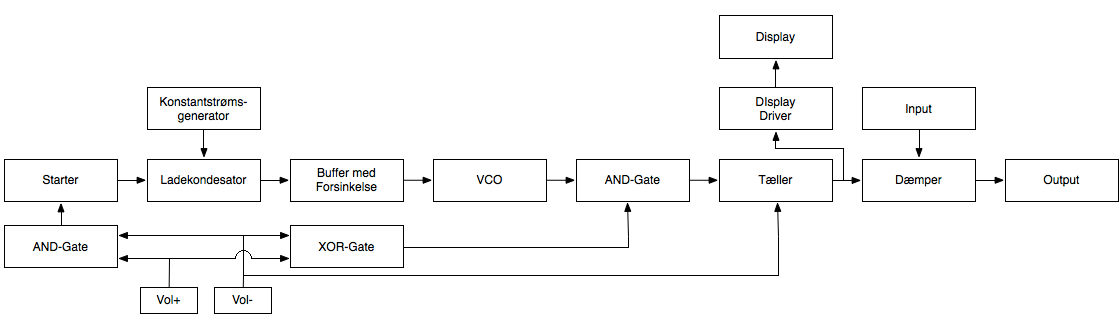
\includegraphics[width=\textwidth]{teknisk/volumenkontrol/blokdiagram.png}
\caption{Blokdiagram over volumenkontrollen}
\label{fig:volumenkontrol_opbygning}
\end{figure}

\subsection{Simulering}
\label{volumenkontrol-simulering}

\begin{figure}[h]
\centering
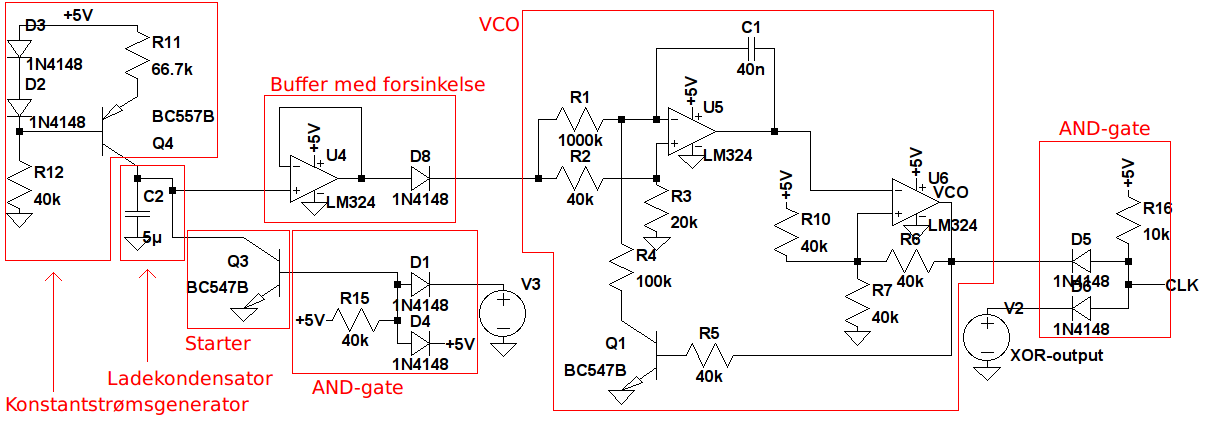
\includegraphics[width=\textwidth]{teknisk/volumenkontrol/diagram.png}
\caption{Diagram over volumenkontrollen}
\label{fig:volumenkontrol_diagram}
\end{figure}

\subsubsection{Konstantstrømsgenerator}
\label{volumenkontrol-simulering-konstantstroemsgenerator}

Konstantstrømsgeneratorens opgave er at leve en konstant strøm, denne strøm bruges til at oplade en kondensator (ladekondensatoren). Diagrammet er vist på figur \ref{fig:volumenkontrol_konstantstroemsgenerator_diagram}. Når en kondensator lades med en konstant strøm, vil spændingen over den stige lineært, dette fremgår også af ligning \ref{equ:konstantstroemsgenerator1}.

\begin{equation}
\label{equ:konstantstroemsgenerator1}
V = \frac{I \cdot t}{C}
\end{equation}

Konstantstrømsgeneratoren er designet med udgangs på at der vil være et spændingsfald på $0,5 V$ over $D_2$, $D_3$, $R_{11}$ og $Q_{4_{BE}}$. I databladet for 1N4148 fremgår det at den vil have en $V_F$ spændingen på $0,5 V$ ved en $I_F$ strøm på $0,1 mA$. Spændingen over modstanden $R_{12}$ er således givet ved ligningen \ref{equ:konstantstroemsgenerator2}.

\begin{equation}
\label{equ:konstantstroemsgenerator2}
U_{R_{12}} = \frac{V_{CC} - 2 \cdot V_F}{I_F} = \frac{5V - 2 \cdot 0,5 V}{0,1 mA} = 40 k\ohm
\end{equation}

Den kondensator som konstantstrømsgeneratoren kaldes ladekondensatoren, denne har en kapacitet på $5 \mu F$ og den ønskede oplade tid er $3 s$. Kondensatoren oplades fra 0 V til $V_{CC} - V_F = 4,5 V$, hvor $V_F$ er spændingen over én diode. Udfra disse to ting kan den konstante strøm, $I_{konst}$, nu beregnes, se ligning \ref{equ:konstantstroemsgenerator3}.

\begin{equation}
\label{equ:konstantstroemsgenerator3}
V_{CC} - V_F = \frac{I_{konst} \cdot t}{C} \Rightarrow 4,5 V = \frac{I_{konst} \cdot 3 s}{5 \mu F} \Rightarrow I_{konst} = 7,5 \mu A
\end{equation}

Spændingen over $R_{11}$ er, som tidligere nævnt, $0,5 V$ og strømmen igennem den er $I_{konst}$, der kan Ohms lov bruges til at beregne modstanden, se ligning \ref{equ:konstantstroemsgenerator4}.

\begin{equation}
\label{equ:konstantstroemsgenerator4}
V = R \cdot I = 0,5 V = R \cdot 7,5 \mu A \Rightarrow R = 66,7 k\ohm
\end{equation}

\subsubsection{Starter}
\label{volumenkontrol-simulering-starter}

Starterens opgave er at holde spændingen over ladekondensatoren på $0 V$, når der ikke trykkes på en af volumenknapperne. Dette gøres ved at lede al den strøm som konstantstrømsgeneratoren levere til stel.

\subsection{Accepttest}
\label{volumenkontrol-accepttest}